% !TeX program = pdflatex
% =============================================================================
% Aufgabenblatt: Magnetfelder
% UZH Praktikum I -- Sara Romer Urban, Kantonsschule im Lee, HS2026
% Klasse: 4fh (01.09.2026, nur 4fh).
%
% Uebungsaufgaben fuer die Vor-/Nachbereitung, zusammengestellt aus:
%   - Bilder/magnetfelder_zeichnen_aufgabe(.png/_loesung.png) und
%     Bilder/magnetfelder_stabmagnet_aufgabe.png (bereits im Themenordner
%     vorhanden, von Loris bereitgestellt).
%   - den LEIFIphysik-PDFs in diesem Ordner ("Magnetische Flussdichte in der
%     Umgebung von geraden Leitern - Formelumstellung", "Magnetische
%     Flussdichte im Innenraum von luftgefuellten Zylinderspulen -
%     Formelumstellung", "Spulenstrom fuer ein Magnetfeld", "Magnetfeld
%     einer Ringspule") -- Aufgabentexte und Zahlenwerte von dort
%     uebernommen, Loesungswege selbst nachvollzogen und ausformuliert.
% Nach Schwierigkeit geordnet (leicht -> mittelschwer, gemaess LEIFIphysik-
% Einstufung bzw. eigener Einschaetzung fuer die beiden Bildaufgaben) und
% mit explizitem Schwierigkeitsgrad-Vermerk (\Schwierigkeit-Makro) direkt
% unter jedem Aufgabentitel.
%
% Stand 03.09.2026: Aufgaben 3, 5, 6, 7 zur magnetischen Flussdichte
% ueberarbeitet, damit dieselbe Rechenoperation (nach B, N bzw. I umstellen)
% nicht mehrfach identisch wiederholt wird -- jede Aufgabe testet jetzt eine
% andere Faehigkeit: Aufgabe 3 direktes Einsetzen (nach B) UND eine
% Verstaendnisfrage zur Proportionalitaet (ohne zu rechnen); Aufgabe 4 (neu)
% Oersted-Versuch fuer beide Stromrichtungen skizzieren; Aufgabe 5 Umstellen
% nach N; Aufgabe 6 Skalierungs-Verstaendnis (die Weicheisenkern-Frage wurde
% entfernt, da im Unterricht nicht behandelt); Aufgabe 7 (Zusatz) Polung per
% Rechte-Faust-Regel UND Umstellen nach I. Alle Formelumstellungs-Zahlenwerte
% verwenden bewusst Nicht-SI-Einheiten (mA, mm, nT, µT), sodass zuerst ins
% SI-System umgerechnet werden muss -- die Formelsammlung nennt dafuer jetzt
% auch die relevanten SI-Vorsilben (Milli/Mikro/Nano) oben, nicht nur die
% Zieleinheit je Symbol.
%
% Hinweis: Ringspule (Aufgabe 7) ist im aktuellen Arbeitsblatt
% (arbeitsblatt5-magnetfelder.tex) NICHT enthalten (siehe dessen
% Header-Kommentar) -- hier als Zusatz-/Vertiefungsaufgabe aufgenommen, weil
% sie dieselbe Spulenformel verwendet und im Quellmaterial vorlag; ein
% kurzer Erklaersatz brueckt die fehlende Theorie direkt in der Aufgabe. Die
% Weicheisenkern-Frage (frueher Aufgabe 5, zweite Verstaendnisfrage) wurde
% ganz gestrichen (Stand 03.09.2026), da Permeabilitaet/Weicheisenkern auch
% im Unterricht nicht behandelt wurde -- entsprechend auch die
% Kernmaterial-Formel aus der Formelsammlung entfernt.
%
% Aufgabe 2 (Stabmagnet-Polung): Die Loesung ist aus dem Feldlinienmuster
% erschlossen (glatter Uebergang = Anziehung/entgegengesetzte Orientierung,
% Sattelpunkt mit auseinanderweichenden Linien = Abstossung/gleiche
% Orientierung) -- Loris bitte anhand des Originalbilds gegenpruefen, bevor
% dies als Loesungsschluessel verwendet wird.
% =============================================================================
\documentclass[addpoints,11pt,a4paper]{exam}

\usepackage[T1]{fontenc}
\usepackage[utf8]{inputenc}
\usepackage[ngerman]{babel}
\usepackage{lmodern}
\usepackage[a4paper,margin=2.2cm,headheight=14pt]{geometry}
\usepackage{amsmath}
\usepackage{amssymb}
\usepackage{siunitx}
% Hausstil: zusammengesetzte Einheiten immer als echter Bruch (\frac), nicht
% als Inline-Schrägstrich oder \tfrac -- gilt global für jedes \si/\SI.
\sisetup{per-mode=fraction,fraction-command=\frac}
\usepackage{array,booktabs,tabularx,multirow}
\usepackage{enumitem}
\usepackage{xcolor}
\usepackage{colortbl}
\usepackage{tikz}
\usepackage{physics}
\usepackage{circuitikz}
\usepackage[most]{tcolorbox}
\usepackage{lastpage}
\usepackage{graphicx}
\usepackage{hyperref}

\usetikzlibrary{arrows.meta,calc,angles,quotes,decorations.markings}

\usepackage{setspace}
\usepackage{needspace}
\setlength{\parindent}{0pt}
\setlength{\parskip}{0.6em}
\setstretch{1.08}
\setlist[itemize]{itemsep=0.4em}

% -----------------------------
% Farben (Corporate-Farbschema Physik KFR)
% -----------------------------
\definecolor{titleblue}{HTML}{183A6B}
\definecolor{accentblue}{HTML}{2E6F9E}
\definecolor{lightblue}{HTML}{EAF4FB}
\definecolor{verylightblue}{HTML}{F7FBFE}
\definecolor{lightgray}{HTML}{F4F6F8}
\definecolor{darkgray}{HTML}{4A4A4A}
\definecolor{accentorange}{HTML}{D9720C}
\definecolor{accentpurple}{HTML}{7B2D8E}
\definecolor{lightorange}{HTML}{FCEEE0}
\definecolor{lightpurple}{HTML}{F3EAF7}

% Links (hyperref): farblich ans Corporate-Farbschema angeglichen.
\hypersetup{
  colorlinks=true,
  urlcolor=accentblue,
  linkcolor=accentblue,
  pdftitle={Aufgabenblatt 4: Magnetfelder},
  pdfauthor={Loris Keller}
}

% -----------------------------
% Spaltentypen
% -----------------------------
\newcolumntype{Y}{>{\centering\arraybackslash}X}
\newcolumntype{P}[1]{>{\raggedright\arraybackslash}p{#1}}

% -----------------------------
% Boxen
% -----------------------------
\tcbset{before skip=10pt, after skip=10pt}
\newtcolorbox{titlebox}{
  enhanced,
  colback=titleblue,
  colframe=titleblue,
  boxrule=0pt,
  arc=3mm,
  left=3mm,right=3mm,top=3mm,bottom=3mm
}

\newlength{\aufgabenindent}
\settowidth{\aufgabenindent}{10.\hskip\labelsep}

% Praktikum I: keine farbigen Rahmen fuer Fliesstext-Boxen (nur Formel-,
% Hinweis- und Antwortbox bleiben Boxen) -- siehe
% institutionen/UZH-Praktikum-I/CLAUDE.md, Abschnitt "Boxen-Layout".
\newtcolorbox{taskbox}[1][]{
  enhanced, breakable,
  colback=white, colframe=white, boxrule=0pt,
  left=0mm,right=0mm,top=0mm,bottom=0mm,
  before skip=10pt, after skip=10pt,
  before upper={%
    \def\tmpboxtitle{#1}%
    \ifx\tmpboxtitle\empty\else\noindent\textbf{#1}\par\smallskip\fi
  }
}

% formelbox: Violett, um die zentralen Formeln dieser Einheit hervorzuheben.
\newtcolorbox{formelbox}[1][Formel]{
  enhanced,
  breakable,
  colback=lightpurple,
  colframe=accentpurple,
  title={#1},
  fonttitle=\bfseries,
  boxrule=0.9pt,
  arc=2mm,
  left=5mm,right=5mm,top=2mm,bottom=2mm
}

% hinweisbox: Orange, für wichtige Klarstellungen/Verwechslungswarnungen.
\newtcolorbox{hinweisbox}[1][Hinweis]{
  enhanced,
  breakable,
  colback=lightorange,
  colframe=accentorange,
  title={#1},
  fonttitle=\bfseries,
  boxrule=0.7pt,
  arc=2mm,
  left=5mm,right=5mm,top=2mm,bottom=2mm
}

\newtcolorbox{answerbox}{
  breakable,
  colback=white,
  colframe=gray!55,
  boxrule=0.5pt,
  arc=1.5mm,
  left=2mm,right=2mm,top=2mm,bottom=2mm
}

% --- Lösungen ein-/ausblenden -----------------------------------------------
\noprintanswers
%\printanswers

\pointformat{}
\renewcommand{\solutiontitle}{\noindent\color{titleblue}\textbf{Lösung:}\enspace}

\pagestyle{headandfoot}
\cfoot{\textcolor{darkgray}{Seite \thepage\ von \pageref{LastPage}}}

\newcommand{\Kopfzeile}[4]{%
  \begin{titlebox}
    {\color{white}\sffamily\bfseries\Large #4}
  \end{titlebox}
  \vspace{0.5em}
  \noindent\textbf{Klasse:}~#1 \hfill \textbf{Datum:}~#2 \hfill \textbf{Thema:}~#3
    \hfill \textbf{Lehrperson:}~Loris Keller
  \vspace{0.8em}
  \lhead{\textcolor{darkgray}{#3}}
  \rhead{\textcolor{darkgray}{#4}}
}

\newlength{\antwortraumlen}
\newcommand{\Antwortraum}[1]{%
  \pgfmathsetlength{\antwortraumlen}{#1*2.5cm}%
  \begin{answerbox}
    \rule{0pt}{\antwortraumlen}%
  \end{answerbox}%
}

% Schwierigkeitsgrad: kurze Einstufung direkt unter dem Aufgabentitel, wie
% auf den LEIFIphysik-Quellseiten ("Schwierigkeitsgrad: leichte Aufgabe").
\newcommand{\Schwierigkeit}[1]{%
  \textit{\color{darkgray}Schwierigkeitsgrad: #1}\par\smallskip
}

% Werte für Kopfzeile zentral setzen
\newcommand{\Klasse}{4fh}
\newcommand{\Datum}{01.09.2026}
\newcommand{\Thema}{Magnetfelder}
\newcommand{\ArbeitsblattTitel}{Aufgabenblatt 4: Magnetfelder}

\begin{document}

\Kopfzeile{\Klasse}{\Datum}{\Thema}{\ArbeitsblattTitel}

% =============================================================================
% Formelsammlung
% =============================================================================
\begin{formelbox}[Formelsammlung]
Vorsilben (zuerst in SI-Einheiten umrechnen!): $1\,\text{m}X=10^{-3}\,X$
(Milli), $1\,\mu X=10^{-6}\,X$ (Mikro), $1\,\text{n}X=10^{-9}\,X$ (Nano).
\begin{align*}
  B &= \frac{\mu_0}{2\pi}\cdot\frac{I}{r} &&\text{gerader Leiter, Abstand } r\\
  B &= \mu_0\cdot\frac{N}{l}\cdot I &&\text{Spule, Länge } l\\
  B &= \mu_0\cdot\frac{N}{l}\cdot I &&\text{Ringspule, } l = \pi\cdot d \ (d = \text{mittlerer Durchmesser})
\end{align*}
$\mu_0=4\pi\cdot10^{-7}\,\si{\newton\per\ampere\squared}=1{,}26\cdot10^{-6}\,\si{\newton\per\ampere\squared}$;
$I$ in \si{\ampere}; $r,\,l,\,d$ in \si{\meter}; $N$ dimensionslos; $B$ in
\si{\tesla}.
\end{formelbox}

% =============================================================================
% Aufgabe 1 (leicht): Feldlinien zeichnen
% =============================================================================
\begin{questions}
\begin{taskbox}[Aufgabe 1: Feldlinien zeichnen]
\Schwierigkeit{leicht}
\question Zeichnen Sie für jede der vier Anordnungen die Feldlinien ein.
Bei 3 und 4 zeigt die graue Färbung jeweils denselben Pol wie bei 1 und 2
(vergleichen Sie die Färbung).
\begin{center}
  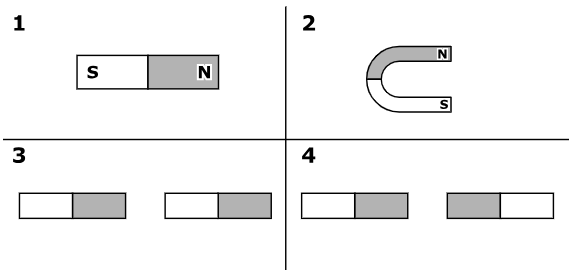
\includegraphics[width=8.5cm]{Bilder/magnetfelder_zeichnen_aufgabe.png}
\end{center}
\Antwortraum{7}
\begin{solution}
\begin{center}
  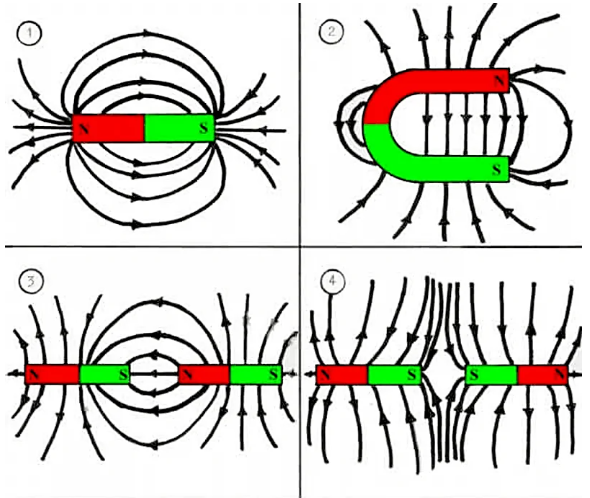
\includegraphics[width=8.5cm]{Bilder/magnetfelder_zeichnen_aufgabe_loesung.png}
\end{center}
Bei 3 (ungleichnamige Pole zueinander) verbinden sich die Feldlinien
durchgehend zwischen den beiden Magneten. Bei 4 (gleichnamige Pole
zueinander) stossen sich die Felder ab, die Feldlinien weichen im
Zwischenraum auseinander.
\end{solution}
\end{taskbox}
\end{questions}

% =============================================================================
% Aufgabe 2 (leicht): Polung eines Stabmagneten bestimmen
% =============================================================================
\begin{questions}
\begin{taskbox}[Aufgabe 2: Polung bestimmen]
\Schwierigkeit{mittel}
\question Der obere Stabmagnet ist bekannt gepolt (N/S beschriftet), der
untere (\glqq ?\grqq{}) nicht. Bestimmen Sie für beide abgebildeten Fälle
anhand des Feldlinienmusters (Eisenfeilspäne), wie der untere Magnet gepolt
sein muss.
\begin{center}
  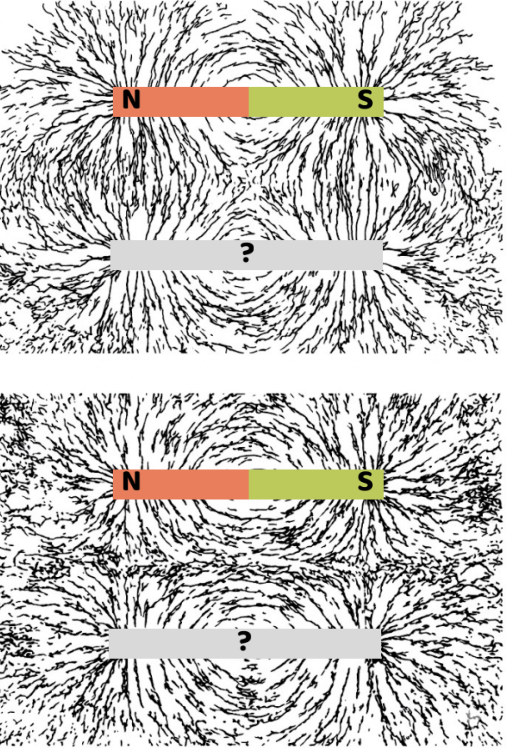
\includegraphics[width=9.5cm]{Bilder/magnetfelder_stabmagnet_aufgabe.png}
\end{center}
\Antwortraum{3}
\begin{solution}
Massgebend ist, ob sich im Zwischenraum ein Sattelpunkt (Feldlinien
weichen auseinander -- Abstossung) oder ein glatter, durchgehender
Übergang (Feldlinien verbinden sich -- Anziehung) zeigt.

\textbf{Oben:} Im Zwischenraum bildet sich ein deutlicher Sattelpunkt, an
dem die Feldlinien auseinanderweichen -- die beiden Magnete stossen sich
ab. Der untere Magnet muss deshalb \emph{spiegelverkehrt} zum oberen
gepolt sein (S links, N rechts).

\textbf{Unten:} Die Feldlinien verbinden sich im Zwischenraum glatt und
durchgehend -- die beiden Magnete ziehen sich an. Der untere Magnet muss
deshalb \emph{gleich} wie der obere gepolt sein (N links, S rechts).
\end{solution}
\end{taskbox}
\end{questions}

% =============================================================================
% Aufgabe 3 (leicht): Gerader Leiter -- Anwendung und Verständnis
% =============================================================================
\begin{questions}
\begin{taskbox}[Aufgabe 3: Gerader Leiter -- Anwendung und Verständnis]
\Schwierigkeit{leicht}
\question[2] Ein unendlich langer, gerader Leiter wird von einem Strom der
Stärke $I=\SI{850}{\milli\ampere}$ durchflossen. Berechnen Sie den Betrag
der magnetischen Flussdichte $B$ in einem Punkt, der $r=\SI{25}{\milli\meter}$
vom Leiter entfernt ist.
\Antwortraum{2}
\begin{solution}
Umrechnen in SI-Einheiten: $I=\SI{850}{\milli\ampere}=\SI{0.850}{\ampere}$,
$r=\SI{25}{\milli\meter}=\SI{0.025}{\meter}$.
\[
  B = \mu_0\cdot\frac{1}{2\pi\cdot r}\cdot I
    = 1{,}26\cdot10^{-6}\,\si{\newton\per\ampere\squared}\cdot\frac{1}{2\pi\cdot\SI{0.025}{\meter}}\cdot\SI{0.850}{\ampere}
    = \SI{6.8e-6}{\tesla}.
\]
\end{solution}

\question[2] Bei welchem der beiden folgenden Fälle ist die magnetische
Flussdichte $B$ grösser -- Fall A (Stromstärke verdoppelt, Abstand
gleich) oder Fall B (Abstand halbiert, Stromstärke gleich)? Begründen Sie
\textbf{ohne zu rechnen}, allein anhand der Formel.
\Antwortraum{2}
\begin{solution}
Beide Fälle ergeben dieselbe Flussdichte $B$: In Fall A verdoppelt sich
$B$, weil $B$ direkt \textbf{\emph{proportional}} zu $I$ ist (doppeltes
$I$ $\to$ doppeltes $B$). In Fall B verdoppelt sich $B$ ebenfalls, weil
$B$ \textbf{\emph{umgekehrt proportional}} zu $r$ ist (halber Abstand
$\to$ doppeltes $B$). Beide Fälle bewirken also denselben Effekt.
\end{solution}
\end{taskbox}
\end{questions}

% =============================================================================
% Aufgabe 4 (leicht): Oersted-Versuch skizzieren
% =============================================================================
\begin{questions}
\begin{taskbox}[Aufgabe 4: Oersted-Versuch skizzieren]
\Schwierigkeit{leicht}
\question[4] Skizzieren Sie den Oersted-Versuch mit dem geraden
Stableiter, von oben betrachtet. Die Batterie ist über zwei Stäbe mit
dem Leiter verbunden: Der Strom fliesst im einen Stab nach oben, im
anderen nach unten -- von oben gesehen kommt der Strom also in einem
Stab aus der Ebene heraus ($\odot$), im anderen fliesst er in die Ebene
hinein ($\otimes$). Zeichnen Sie für \textbf{beide} Batterie-Polungen
das Magnetfeld um \textbf{beide} Stäbe ein: mehrere konzentrische
Kreise, mit Pfeilen, welche die Richtung des Feldes zeigen.
\begin{center}
\begin{minipage}[t]{7.6cm}\centering
\footnotesize Ursprüngliche Polung\\[1mm]
\begin{answerbox}
\vspace{1.8cm}
\begin{center}
\begin{tikzpicture}[>=Latex,thick]
  \begin{scope}[shift={(-1.5,0)}]
    \draw (0,0) circle (0.18);
    \fill (0,0) circle (0.05);
  \end{scope}
  \begin{scope}[shift={(1.5,0)}]
    \draw (0,0) circle (0.18);
    \draw (-0.11,-0.11) -- (0.11,0.11);
    \draw (-0.11,0.11) -- (0.11,-0.11);
  \end{scope}
\end{tikzpicture}
\end{center}
\vspace{1.8cm}
\end{answerbox}
\end{minipage}\hfill
\begin{minipage}[t]{7.6cm}\centering
\footnotesize Batterie umgepolt\\[1mm]
\begin{answerbox}
\vspace{1.8cm}
\begin{center}
\begin{tikzpicture}[>=Latex,thick]
  \begin{scope}[shift={(-1.5,0)}]
    \draw (0,0) circle (0.18);
    \draw (-0.11,-0.11) -- (0.11,0.11);
    \draw (-0.11,0.11) -- (0.11,-0.11);
  \end{scope}
  \begin{scope}[shift={(1.5,0)}]
    \draw (0,0) circle (0.18);
    \fill (0,0) circle (0.05);
  \end{scope}
\end{tikzpicture}
\end{center}
\vspace{1.8cm}
\end{answerbox}
\end{minipage}
\end{center}
\begin{solution}
\begin{center}
\begin{minipage}[t]{6.3cm}\centering
\footnotesize Ursprüngliche Polung\\[1mm]
\begin{tikzpicture}[>=Latex,thick,scale=0.85]
  \begin{scope}[shift={(-1.5,0)}]
    \draw (0,0) circle (0.18);
    \fill (0,0) circle (0.05);
    \foreach \r in {0.5,0.85,1.2}{
      \draw[-{Latex[length=2mm]}] (\r,0) arc (0:75:\r);
    }
  \end{scope}
  \begin{scope}[shift={(1.5,0)}]
    \draw (0,0) circle (0.18);
    \draw (-0.11,-0.11) -- (0.11,0.11);
    \draw (-0.11,0.11) -- (0.11,-0.11);
    \foreach \r in {0.5,0.85,1.2}{
      \draw[-{Latex[length=2mm]}] (\r,0) arc (0:-75:\r);
    }
  \end{scope}
\end{tikzpicture}
\end{minipage}\hfill
\begin{minipage}[t]{6.3cm}\centering
\footnotesize Batterie umgepolt\\[1mm]
\begin{tikzpicture}[>=Latex,thick,scale=0.85]
  \begin{scope}[shift={(-1.5,0)}]
    \draw (0,0) circle (0.18);
    \draw (-0.11,-0.11) -- (0.11,0.11);
    \draw (-0.11,0.11) -- (0.11,-0.11);
    \foreach \r in {0.5,0.85,1.2}{
      \draw[-{Latex[length=2mm]}] (\r,0) arc (0:-75:\r);
    }
  \end{scope}
  \begin{scope}[shift={(1.5,0)}]
    \draw (0,0) circle (0.18);
    \fill (0,0) circle (0.05);
    \foreach \r in {0.5,0.85,1.2}{
      \draw[-{Latex[length=2mm]}] (\r,0) arc (0:75:\r);
    }
  \end{scope}
\end{tikzpicture}
\end{minipage}
\end{center}
Rechte-Faust-Regel, an jedem Stab einzeln angewendet: Zeigt der Daumen in
Stromrichtung, geben die gekrümmten Finger die Feldrichtung an. Beim Stab
mit $\odot$ (Strom kommt zu Ihnen) krümmen sich die Finger \textbf{gegen
den Uhrzeigersinn}. Beim Stab mit $\otimes$ (Strom fliesst von Ihnen weg)
krümmen sich die Finger \textbf{im Uhrzeigersinn}. Beim Umpolen der
Batterie kehrt sich die Stromrichtung in \textbf{beiden} Stäben um --
damit tauschen auch beide Felder ihre Richtung.
\end{solution}
\end{taskbox}
\end{questions}

% =============================================================================
% Aufgabe 5 (leicht): Zylinderspule -- Formelumstellung
% =============================================================================
\begin{questions}
\begin{taskbox}[Aufgabe 5: Zylinderspule -- Formelumstellung]
\Schwierigkeit{leicht}
\question[3] Im Innenraum einer $\SI{35}{\centi\meter}$ langen,
luftgefüllten Spule, durch die ein Strom der Stärke $I=\SI{120}{\milli\ampere}$
fliesst, herrscht ein Feld mit $B=\SI{950}{\micro\tesla}$. Berechnen Sie
die Windungszahl $N$ der Spule.
\Antwortraum{3}
\begin{solution}
Umrechnen in SI-Einheiten: $l=\SI{0.35}{\meter}$,
$I=\SI{120}{\milli\ampere}=\SI{0.120}{\ampere}$,
$B=\SI{950}{\micro\tesla}=\SI{9.50e-4}{\tesla}$.
\[
  B = \mu_0\cdot\frac{N}{l}\cdot I
  \quad\Longrightarrow\quad
  N = \frac{B\cdot l}{\mu_0\cdot I}
\]
\[
  N = \frac{\SI{9.50e-4}{\tesla}\cdot\SI{0.35}{\meter}}{1{,}26\cdot10^{-6}\,\si{\newton\per\ampere\squared}\cdot\SI{0.120}{\ampere}}
    \approx 2200.
\]
\end{solution}
\end{taskbox}
\end{questions}

% =============================================================================
% Aufgabe 6 (mittel): Spule -- Verständnisfragen
% =============================================================================
\begin{questions}
\begin{taskbox}[Aufgabe 6: Spule -- Verständnisfragen]
\Schwierigkeit{mittel}
\question[2] Erläutern Sie, wie sich das Magnetfeld der Spule verändert,
wenn der Strom $I$ verdreifacht und gleichzeitig die Länge $l$ der Spule
halbiert wird (Windungszahl $N$ bleibt gleich).
\Antwortraum{2}
\begin{solution}
\[
  B_{\text{neu}} = \mu_0\cdot\frac{N}{\frac{1}{2}l}\cdot(3I) = 6\cdot\mu_0\cdot\frac{N}{l}\cdot I = 6\cdot B.
\]
Das Magnetfeld versechsfacht sich: Die Verdreifachung von $I$ verdreifacht
$B$, die Halbierung von $l$ verdoppelt $B$ zusätzlich ($3\times2=6$).
\end{solution}
\end{taskbox}
\end{questions}

% =============================================================================
% Aufgabe 7 (mittelschwer): Ringspule
% =============================================================================
\begin{questions}
\begin{taskbox}[Aufgabe 7: Ringspule]
\Schwierigkeit{mittelschwer}
\begin{hinweisbox}[Hinweis]
Biegt man eine lange Zylinderspule zu einem Ring (Ringspule/Torus), gilt
weiterhin $B=\mu_0\cdot\frac{N}{l}\cdot I$ -- nur ist $l$ jetzt nicht mehr
die gerade Spulenlänge, sondern der mittlere Umfang des Rings,
$l=\pi\cdot d$ ($d$ = mittlerer Durchmesser).
\end{hinweisbox}
\question Die Abbildung zeigt eine Ringspule mit mittlerem Durchmesser
$d=\SI{10}{\centi\meter}$.
\begin{center}
  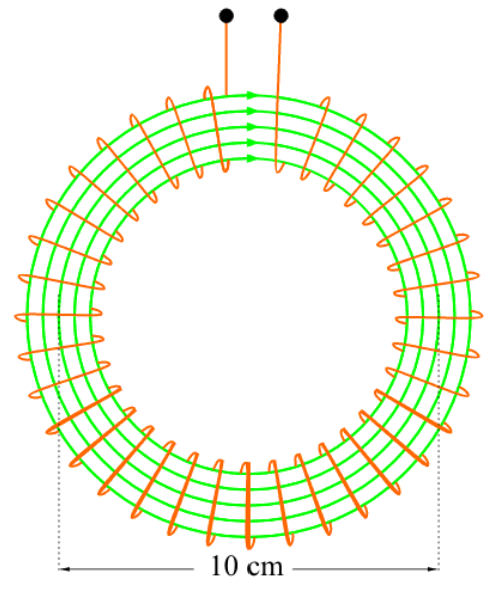
\includegraphics[width=5.5cm]{Bilder/ringspuhle_aufgabe.png}
\end{center}
\begin{parts}
  \part[2] Geben Sie an, wie die Pole der Stromquelle gewählt werden
  müssen, damit sich die eingezeichnete Richtung des Magnetfelds (grüne
  Pfeile) ergibt.
  \Antwortraum{2}
  \begin{solution}
  \begin{center}
    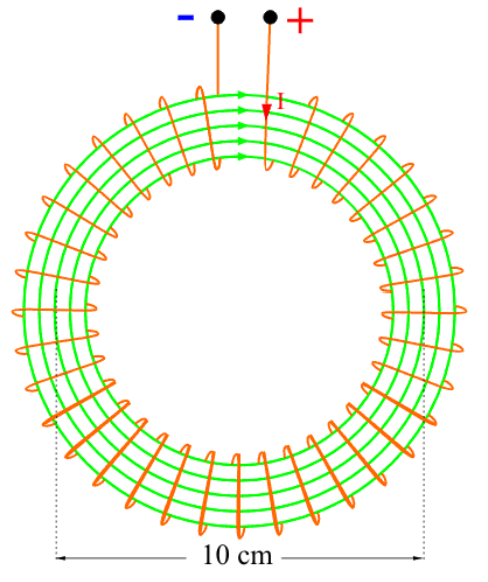
\includegraphics[width=5.5cm]{Bilder/ringspuhle_aufgabe_loesung.png}
  \end{center}
  Mit der Rechte-Faust-Regel für die Spule (Finger in Stromrichtung,
  Daumen zeigt zum \glqq Nordpol\grqq{}, hier: zur eingezeichneten
  Feldrichtung) ergibt sich die oben gezeigte Polung: links Minuspol,
  rechts Pluspol der Stromquelle.
  \end{solution}

  \part[3] Berechnen Sie die Stärke des Stroms, der durch die $N=600$
  Windungen der Ringspule fliessen muss, damit in ihr ein Magnetfeld der
  Flussdichte $B=\SI{6.6}{\milli\tesla}$ herrscht.
  \Antwortraum{3}
  \begin{solution}
  Mit $l=\pi\cdot d$:
  \[
    B = \mu_0\cdot\frac{N}{\pi\cdot d}\cdot I
    \quad\Longrightarrow\quad
    I = \frac{B\cdot\pi\cdot d}{\mu_0\cdot N}
  \]
  \[
    I = \frac{\SI{6.6e-3}{\tesla}\cdot\pi\cdot\SI{0.10}{\meter}}{1{,}26\cdot10^{-6}\,\si{\newton\per\ampere\squared}\cdot 600}
      = \SI{2.7}{\ampere}.
  \]
  \end{solution}
\end{parts}
\end{taskbox}
\end{questions}

\end{document}
